\documentclass[tikz]{standalone}
\usetikzlibrary{positioning}
\usepackage{amsmath}
\usepackage{mathrsfs}

\newcommand{\cat}[1]{\mathscr{#1}}
\newcommand{\obj}[1]{\lowercase{#1}}
\newcommand{\objs}[1]{#1}
\newcommand{\mrp}[3]{{#1}:{#2}\to{#3}}
\newcommand{\mrps}[3]{#1(#2,#3)}
\newcommand{\id}[1]{\mathrm{id}_{#1}}
\newcommand{\op}[1]{{#1}^{\mathrm{op}}}
\newcommand{\set}{\mathbf{Set}}
\newcommand{\Top}{\mathsf{Top}}
\newcommand{\blat}{\mathsf{BLat}}
\newcommand{\stone}{\mathsf{Stone}}
\DeclareMathOperator{\dom}{dom}
\DeclareMathOperator{\cod}{cod}
\DeclareMathOperator{\colim}{Colim}
\DeclareMathOperator{\lan}{Lan}
\DeclareMathOperator{\ran}{Ran}
\DeclareMathOperator{\cone}{Cone}
\DeclareMathOperator{\cocone}{Cocone}


\begin{document}
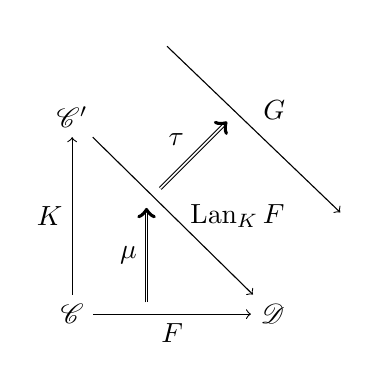
\begin{tikzpicture}
	\def\C{\cat{C}}%
	\def\A{\cat{C'}}%
	\def\D{\cat{D}}%
	\def\K{K}%
	\def\L{\K_!}%
	\def\f{F}%
	\def\g{G}%
	\node (C) {$\A$};
	\node [below=2cm of C] (M) {$\C$};
	\node [right=2cm of M] (A) {$\D$};
	\draw [->] (M) to node [left]         {$\K$}      (C);
	\draw [->] (M) to node [below]        {$\f$}      (A);
	\draw [->] (C) to node [right=0.1cm]  {$\lan_{\K}\f$} (A);
	\node [above right=0.9cm of C] (astart) {};
	\node [below right=2.1cm and 2.2cm of astart] (aend) {};
	\draw [->] (astart) to node [above right] {$\g$} (aend);
	\node [below right=0.65cm and 0.5cm of C] (eend) {};
	\node [below=1.2cm of eend] (estart) {};
	\draw [->,double] (estart) to node [left] {$\mu$} (eend);
	\node [above right=1.1cm and 0.6cm of M] (sstart) {};
	\node [above right=1.2cm of sstart] (send) {};
	\draw [->,double] (sstart) to node [above left] {$\tau$} (send);
\end{tikzpicture}
\end{document}
